\section{App auf Rezept}
Wie bereits erwähnt würde am 19.Dezember 2019 mit der Inkraftsetzung des DVG\footnote{Digitalen-Versorgungs-Gesetzes}, die ``App auf Rezept'' für Patientinnen und Patienten in die Gesundheitsverordnung eingeführt. DiGA\footnote{Digitale Gesundheitsanwendung} können somit von Ärzten und Psychotherapeuten verordnet und durch die Krankenkasse erstattet werden. Dies eröffnet vielfältige Möglichkeiten, um bei der Erkennung und Behandlung von Krankheiten sowie auf dem Weg zu einer selbstbestimmten gesundheitsförderlichen Lebensführung zu unterstützen.

``Das BfArM\footnote{Bundesinstitut für Arzneimittel und Medizinprodukte} hat diesen bedeutenden Baustein der Digitalisierungsstrategie der Bundesregierung und des Bundesgesundheitsministeriums von Anfang an mitgestaltet und unterstützt Hersteller und Anwender digitaler Medizinprodukte wie z.B. Medical Apps seit Jahren intensiv u.a. bei Fragen zur Einstufung einer App als Medizinprodukt oder zur Cybersicherheit von Medizinprodukten.''~\cite{bfarm}

``Das Bundesinstitut für Arzneimittel und Medizinprodukte (BfArM) ist eine selbstständige Bundesoberbehörde im Geschäftsbereich des Bundesministeriums für Gesundheit (BMG). Es hat in diesem Kontext die Aufgabe, Anträge zur Aufnahme von DiGA in das Verzeichnis wissenschaftlich zu bewerten. Es stellt außerdem das Verzeichnis für digitale Medizinprodukte bereit, die nach erfolgreicher Prüfung als erstattungsfähige digitale Gesundheitsanwendungen (DiGA) gelistet werden.''~\cite{bfarm}

Über sogenannte ``Bekanntmachungen'' im Bundesanzeiger, die erstmals am~\textit{06.1.2020}~\cite{bekanntmachungen061020} und zuletzt am \textit{29.12.2020}~\cite{bekanntmachungen291220} erschienen ist, werden Informationen wie die Errichtung des Verzeichnisses für digitale Gesundheitsanwendungen (DiGA), die Bildung neuer Gruppen oder die Veränderung bestehender Gruppen im DiGA-Verzeichnis, die Aufnahme neuer DiGA im DiGA-Verzeichnis, die Streichung von DiGA aus dem DiGA-Verzeichnis veröffentlicht. Diese Veröffentlichung folgt vierteljährlich.

Für ärztliche oder psychotherapeutische Leistungserbringer eröffnet das Verzeichnis vielfältige Möglichkeiten, sich einen Überblick über verfügbare DiGA zu verschaffen, die möglicherweise für ihre Patienten infrage kommen könnten. Die im Verzeichnis aufgeführten Informationen sollen das gemeinsame aussuchen mit dem Patienten, unterstützen. Sodass die zur aktuellen Situation am besten geeignete DiGA verordnet werden kann.

\subsection{Wie kann eine DiGA verordnet werden?}
Im Verzeichnis findet man wichtige Informationen, die unmittelbar zur Verordnung einer ausgewählten Verordnungs Einheit (DiGA-VE) der erstattungsfähigen DiGA\footnote{Digitale Gesundheitsanwendung} für einen Patienten mit vorliegender Indikation genutzt werden kann.
Die wesentlichen Verordnung relevanten Informationen werden, ggfs. mit einem gewissen, technisch bedingten Zeitverzug, auch von dem Praxisverwaltungssystemhersteller unmittelbar in der Praxisverwaltungssystem (PVS) bereitgestellt.
Schlüssel zur Verordnung einer bestimmten DiGA-VE\footnote{Verordnungseinheit - Ein bestimmtes DiGA-Modul für einen bestimmten Verordnungszeitraum} ist, analog zur unterschiedlichen Dosierungen und Packungsgrößen bei Arzneimitteln, die Pharmazentralnummer (PZN), die dazu auf dem Verordnungsvordruck aufzufinden ist ,anzugeben. Man beachte diesbezüglich die Hinweise z.B. der Kassenärztliche Bundesvereinigung (KBV) sowie ggfs. des PVS-Herstellers.
Zu jeder DiGA wird im Verzeichnis auf der Informationsseite für Leistungserbringer u.a. eine Tabelle vorgesehener Verordnungseinheiten einschließlich der jeweiligen Eigenschaften und der zugehörigen PZN angegeben.

Das BfArM\footnote{Bundesinstitut für Arzneimittel und Medizinprodukte} ist nicht in den Verordnungs- beziehungsweise Erstattungsprozess für DiGA eingebunden, hier sind nur der Patient, Arzt oder Therapeut und die Gesetzlichen Krankenversicherungen eingeschlossen, wie auf Abbildung\ref{fig:verordnungsprozess} zu erkennen ist.
Nachdem die passende Verordnungseinheit einer DiGA mit der entsprechenden PZN\footnote{Pharmazentralnummer} auf einem üblichen Kassenrezept verordnet wurde, kann der Patient dieses bei seiner gesetzlichen Krankenkasse einreichen und um Zusendung eines Freischaltcodes für die DiGA bitten. Dieser wird ihm dann von der Krankenkasse zugesandt einschließlich weiterer Hinweise, unter welchem Link die DiGA heruntergeladen oder der Hersteller der DiGA dazu kontaktiert werden kann z.B. falls es zusätzliche Hardware Bestandteil der DiGA gibt.
Nach der Aktivierung der DiGA unter Nutzung des Freischaltcodes kann die DiGA für den verordneten Zeitraum genutzt werden und der DiGA-Hersteller rechnet die Kosten unter Bezug auf den verwendeten Freischaltcode direkt mit der Krankenkasse ab.~\cite{digaLeistungserbringer}
\begin{figure}[H]
	\centering
	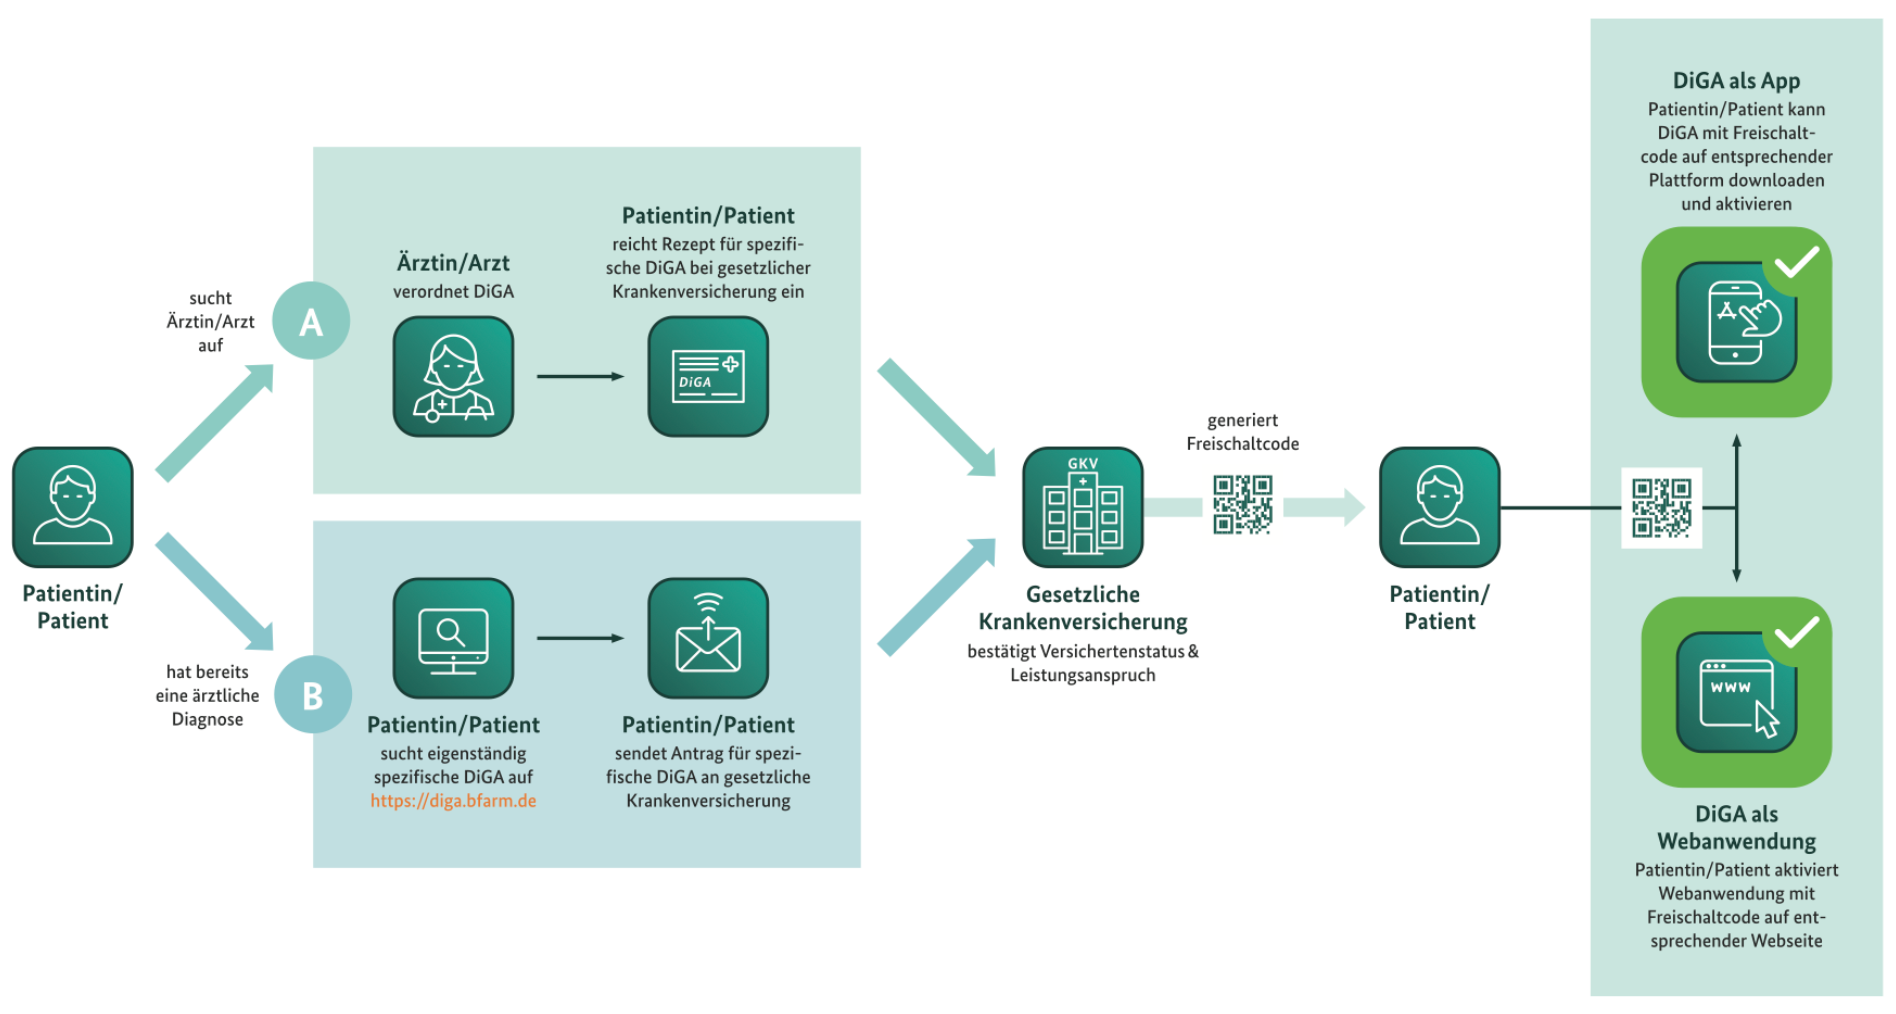
\includegraphics[width=450px, keepaspectratio]{assets/verordnungs_prozess.png}
	\caption[Verordnungs- und Erstattungsprozess]{Verordnungs- und Erstattungsprozess,~Quelle:~\cite{digaLeistungserbringer}}
	\label{fig:verordnungsprozess}
\end{figure}


\subsection{Wie funktioniert das Fast-Track- Verfahren?}
Wie bereits oben genannt, muss der Hersteller zur Prüfung durch das BfArM\footnote{Bundesinstitut für Arzneimittel und Medizinprodukte} einen Antrag zur Aufnahme einer DiGA\footnote{Digitale Gesundheitsanwendung} in das DiGA-Verzeichnis stellen, sodass dann das Anliegen und ob diese den Voraussetzungen entspricht geprüft werden. Die gestellten Anforderungen an die DiGA beziehen sich auf die Sicherheit, Qualität, Verwendbarkeit, Interoperabilität, Datensicherheit und den Datenschutz.
Was jedoch ebenso von großer Relevanz ist, ist dass die positiven Versorgungseffekte, wie der medizinische Nutzen und die Verfahrens- und Strukturverbesserungen gewährleistet werden können.
Anhand der Prüfung wird entschieden, ob die DiGA direkt abgelehnt, bei halb erkennbarem Genügen in die vorläufige Aufnahme zur weiteren Testung während des Verfahrens geschickt oder direkt bestätigt und eingetragen wird.
Falls die DiGA nur teilweise den Voraussetzungen entspricht, wird sie vorläufig in das DiGA-Verzeichnis aufgenommen, muss jedoch eine ca. 12 monatige Erprobungsphase durchlaufen. Nach Abschluss des Verfahrens erhält der Hersteller einen Entscheid, ob seine DiGA die Voraussetzungen zur Aufnahme in das DiGA-Verzeichnis erfüllt. 
In der Abbildung~\ref{fig:fasttrackverfahren} sind die einzelnen Vorkehrungen des Prozesses dargestellt.~\cite{digahersteller}

\begin{figure}[H]
	\centering
	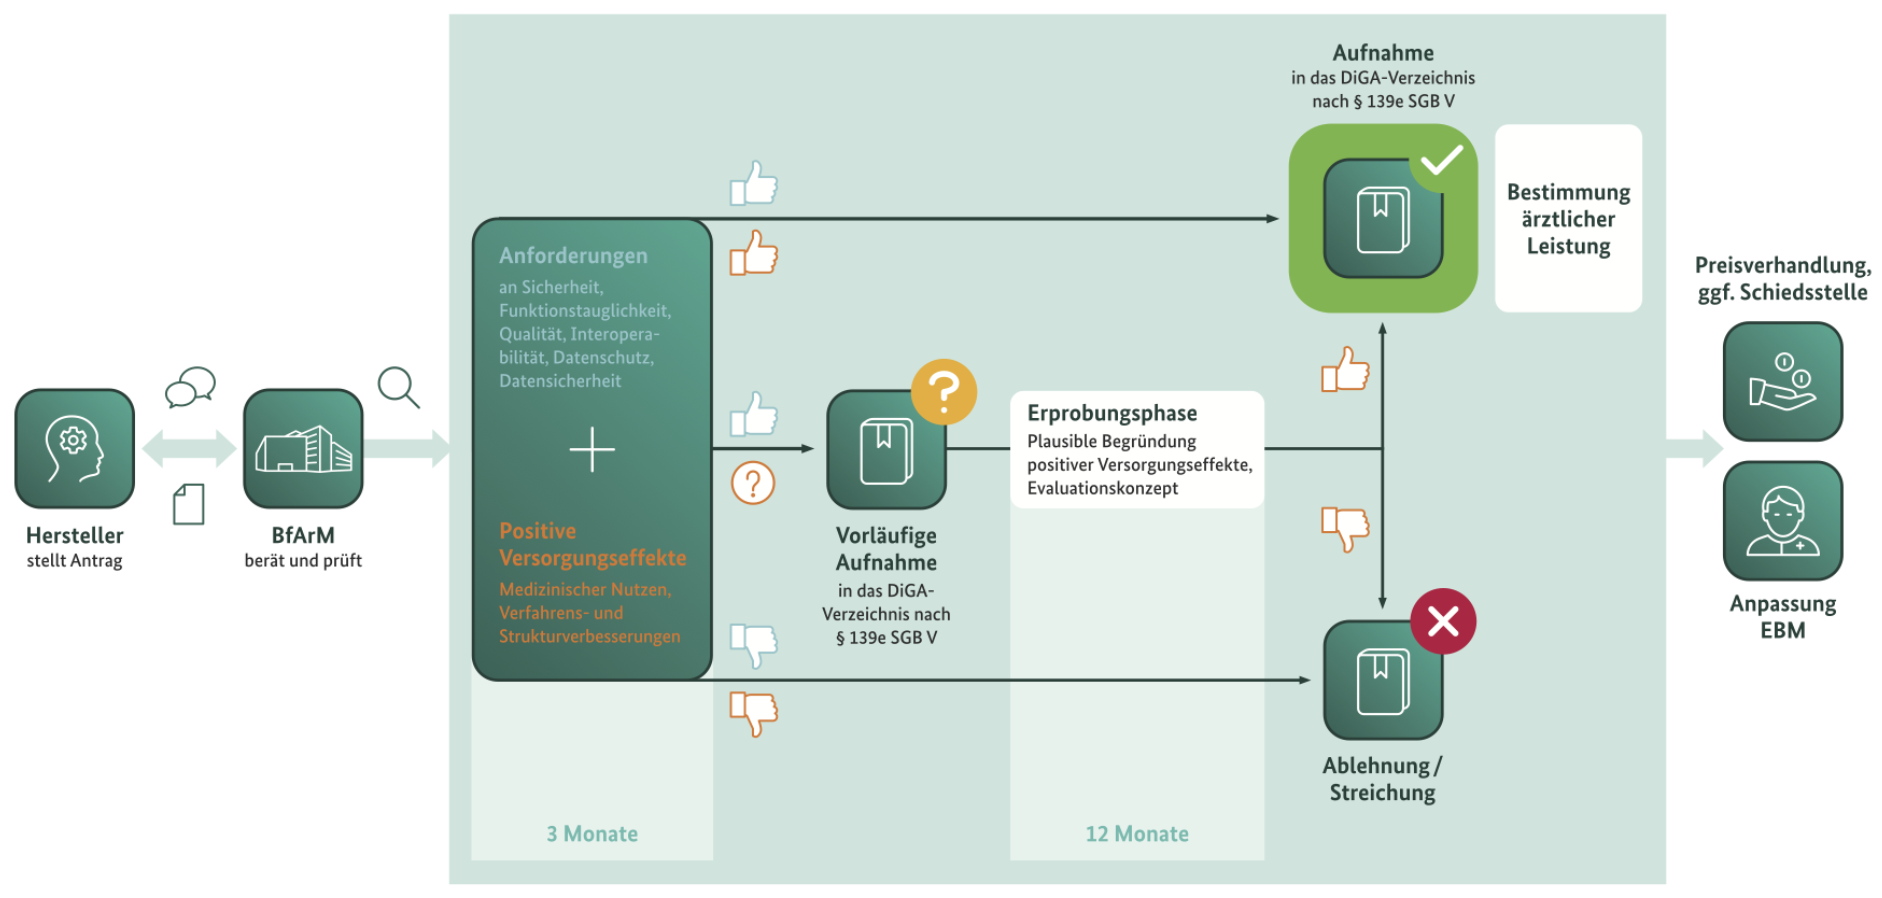
\includegraphics[width=450px, keepaspectratio]{assets/fastTrack_prozess.png}
	\caption[Fast-Track-Verfahren]{Fast-Track-Verfahren,~Quelle:~\cite{digahersteller}}
	\label{fig:fasttrackverfahren}
\end{figure}

\subsection{Das DiGA Verzeichnis}
Das~\textit{DiGA-Verzeichnis}~\cite{digaverzeichnis} des Bundesministerium für Arzneimittel und Medizinprodukte ist ein kürzlich zur Verfügung gestelltes System. Nach Antrag zur Aufnahme in das Verzeichnis und erfolgreichen durchlaufen des Fast-Track Verfahrens, werden die digitalen Gesundheitsanwendungen, also z.B. Apps oder browserbasierte Anwendungen im Verzeichnis aufgelistet. Alle hier hinterlegten Anwendungen sind ``als Medizinprodukt mit niedrigem Risiko CE-zertifiziert, zusätzlich vom BfArM als DiGA geprüft und können damit vom Arzt verschrieben oder bei entsprechender Diagnose direkt von gesetzlichen Krankenkassen erstattet werden.'' ~\cite{digaNutzer}
Patienten finden hier hilfreiche Informationen zu den Eigenschaften und den Leistungen der DiGA, Information zum Nutzen, also wie diese z.B im Alltag zur Verbesserung im Umgang mit einer Erkrankung beitragen können und vieles mehr. Zudem Erfahren Sie hier, wie Ihnen diese vom Arzt oder Psychotherapeuten verschrieben und auf dem Endgerät freigeschaltet werden können.
\begin{figure}[H]
	\centering
	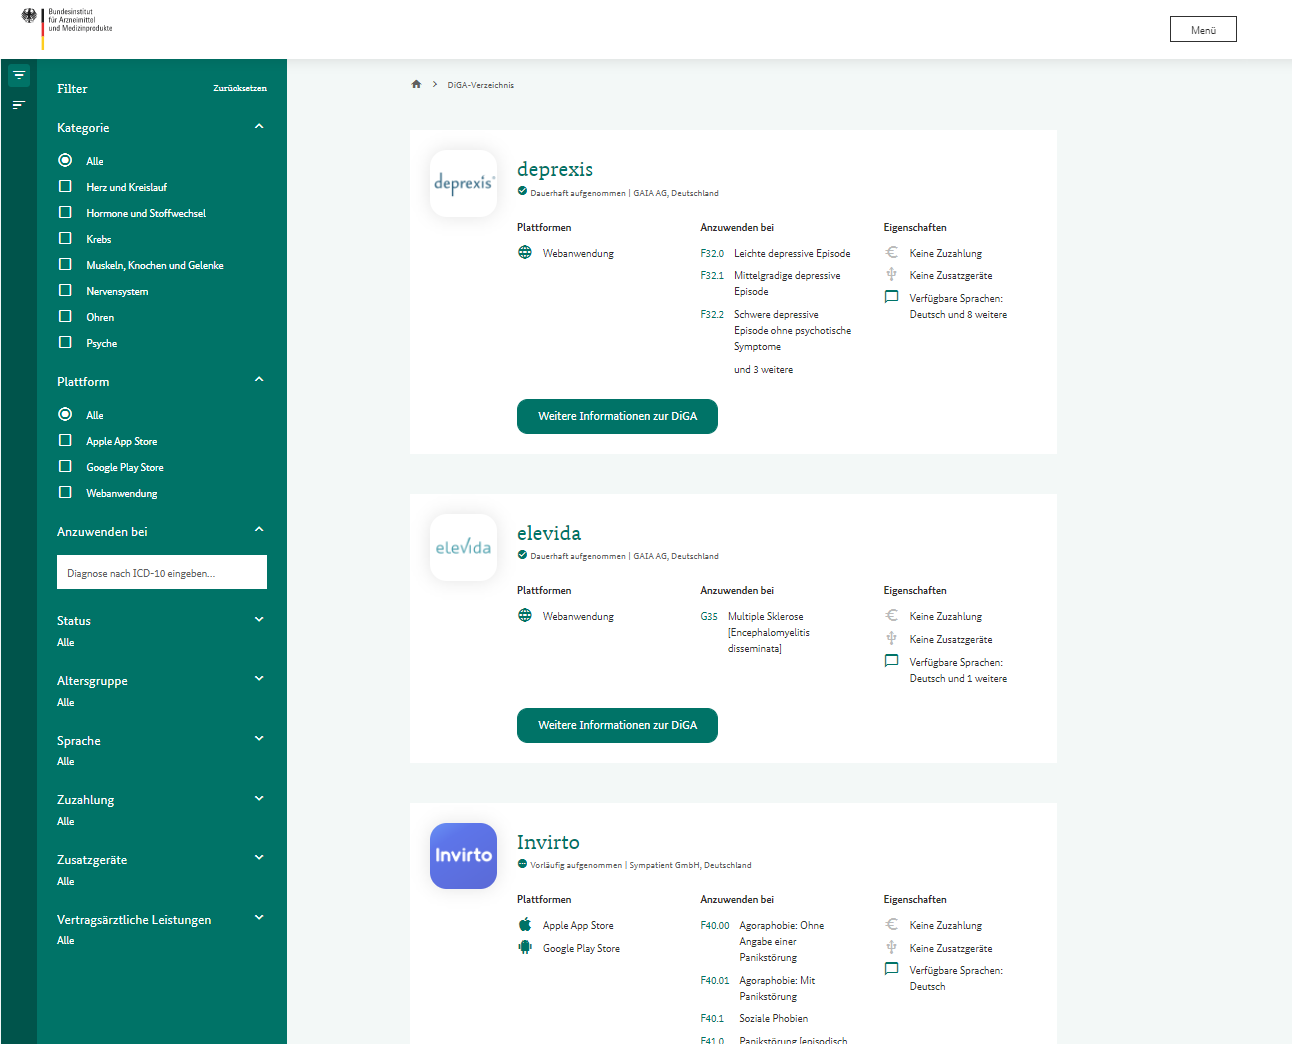
\includegraphics[width=450px, keepaspectratio]{assets/digaVerzeichnis.png}
	\caption[DiGA-Verzeichnis]{DiGA-Verzeichnis,~Quelle:~\cite{digaverzeichnis}}
	\label{fig:digaverzeichnis}
\end{figure}
Das Verzeichnis bietet sehr umfangreiche Informationen zu den einzelnen Gesundheitsanwendungen, welches nicht nur eine Informationsquelle für Patienten bietet sondern auch für Leistungserbringer eine informative Grundlage für Diagnosen oder Verschreibungen ist. Wenn man sich am Beispiel der DiGA ``M-sense Migräne'' die Webseite genauer beleuchtet, entdeckt man viele hilfreich Informationen für beide Seiten. Abbildung \ref{fig:mainTile} zeigt die Informationskarte, die auf der Hauptansicht des DiGA-Verzeichnisses zusehen ist. Jede Anwendung wird so zu nächste kurz und knapp mit den wichtigsten Informationen aufgeführt. Klickt man dann auf ``Weitere Informationen zur DiGA'' gelangt man auf die Detailansicht Abbildung~\ref{fig:detailView}.
\begin{figure}[H]
	\centering
	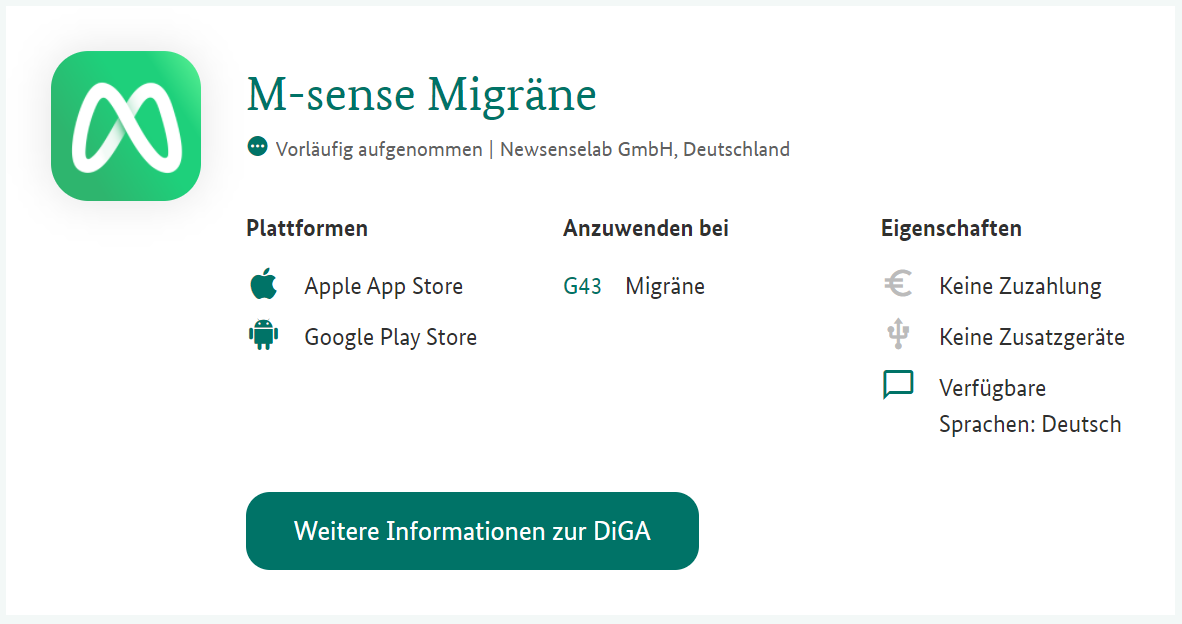
\includegraphics[width=250px, keepaspectratio]{assets/digaBSP1.png}
	\caption[DiGA-Verzeichnis - Kartenansicht]{DiGA-Verzeichnis - Kartenansicht,~Quelle:~\cite{digaverzeichnis}}
	\label{fig:mainTile}
\end{figure}
Auf der Detailansicht angelangt, erhält man genauere Informationen zu dieser Anwendung gegen Migräne. Neben den Eckdaten erfährt man nun weiteres zum Behandlungsprogramm und erhält einen tieferen Einblick in die gesamte Anwendung, wie z. B. über die positiven Versorgungseffekte, zur Datenschutz und Datensicherheit speziell bezogen auf diese Software Abbildung~\ref{fig:foot}.
\begin{figure}[H]
	\centering
	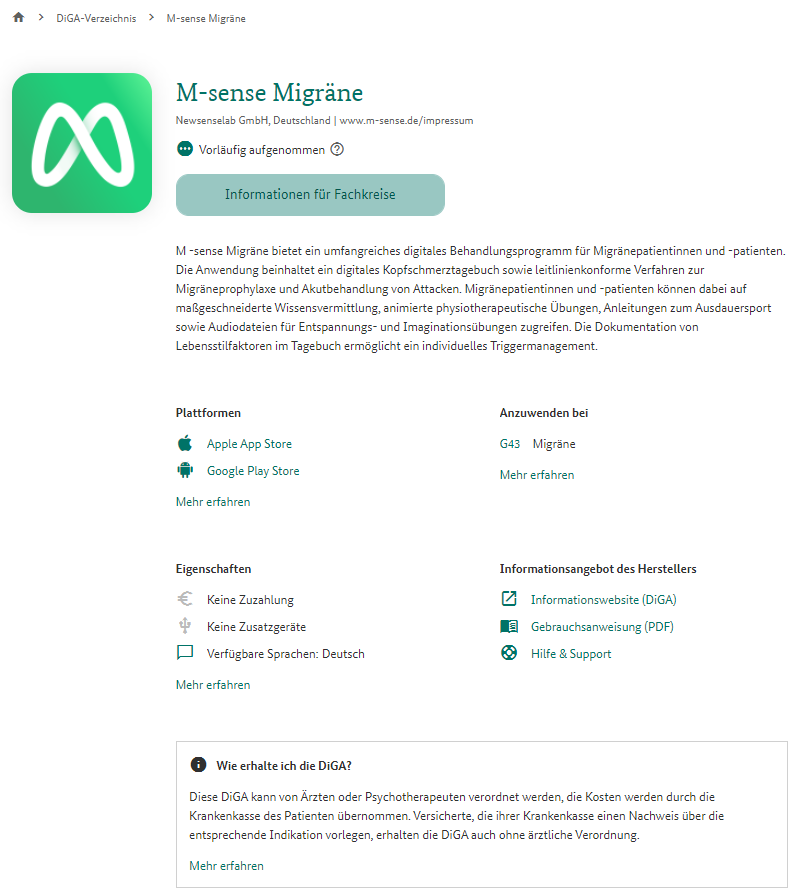
\includegraphics[width=250px]{assets/digaBSP2.png}
	\caption[DiGA-Verzeichnis - Detailansicht]{DiGA-Verzeichnis - Detailansicht,~Quelle:~\cite{digadetailansicht}}
	\label{fig:detailView}
\end{figure}

\begin{figure}[H]
	\centering
	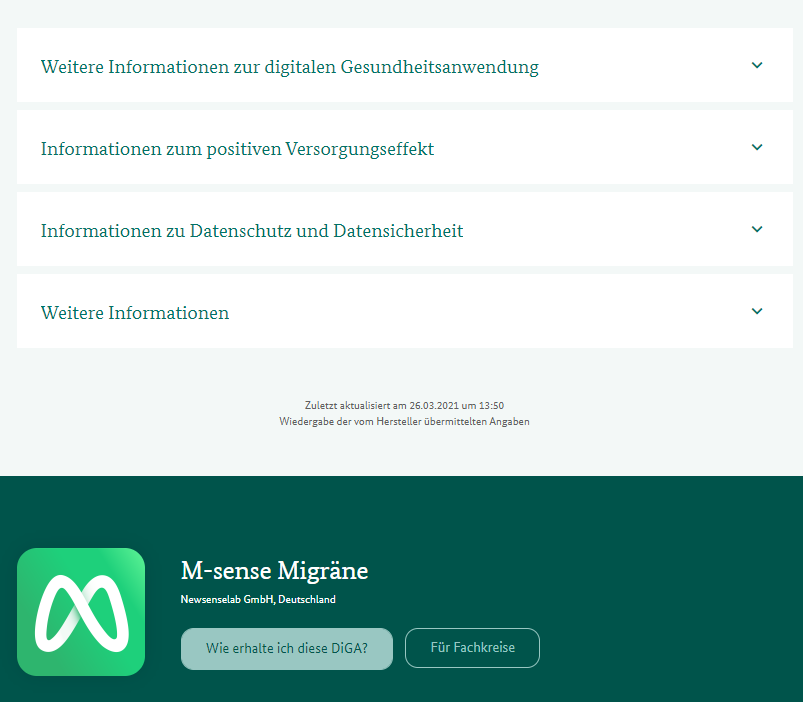
\includegraphics[width=250px]{assets/digaBSP3.png}
	\caption[DiGA-Verzeichnis - Detailansicht]{DiGA-Verzeichnis - Detailansicht,~Quelle:~\cite{digadetailansicht}}
	\label{fig:foot}
\end{figure}

Der gesamte Prozess rund um die DiGA's ist sehr transparent gehalten. Klickt man auf den Button ``Informationen für Fachkreise'' Abbildung~\ref{fig:detailView} erhalten man sogar einen Einblick in die Bewertungsentscheidungen des BfArm bezüglich dieser Anwendung und weitere umfassende Informationen wie z. B. Angaben zur Evidenz, Patientengruppen etc. Abbildung~\ref{fig:moreInfo}.
\begin{figure}[H]
	\centering
	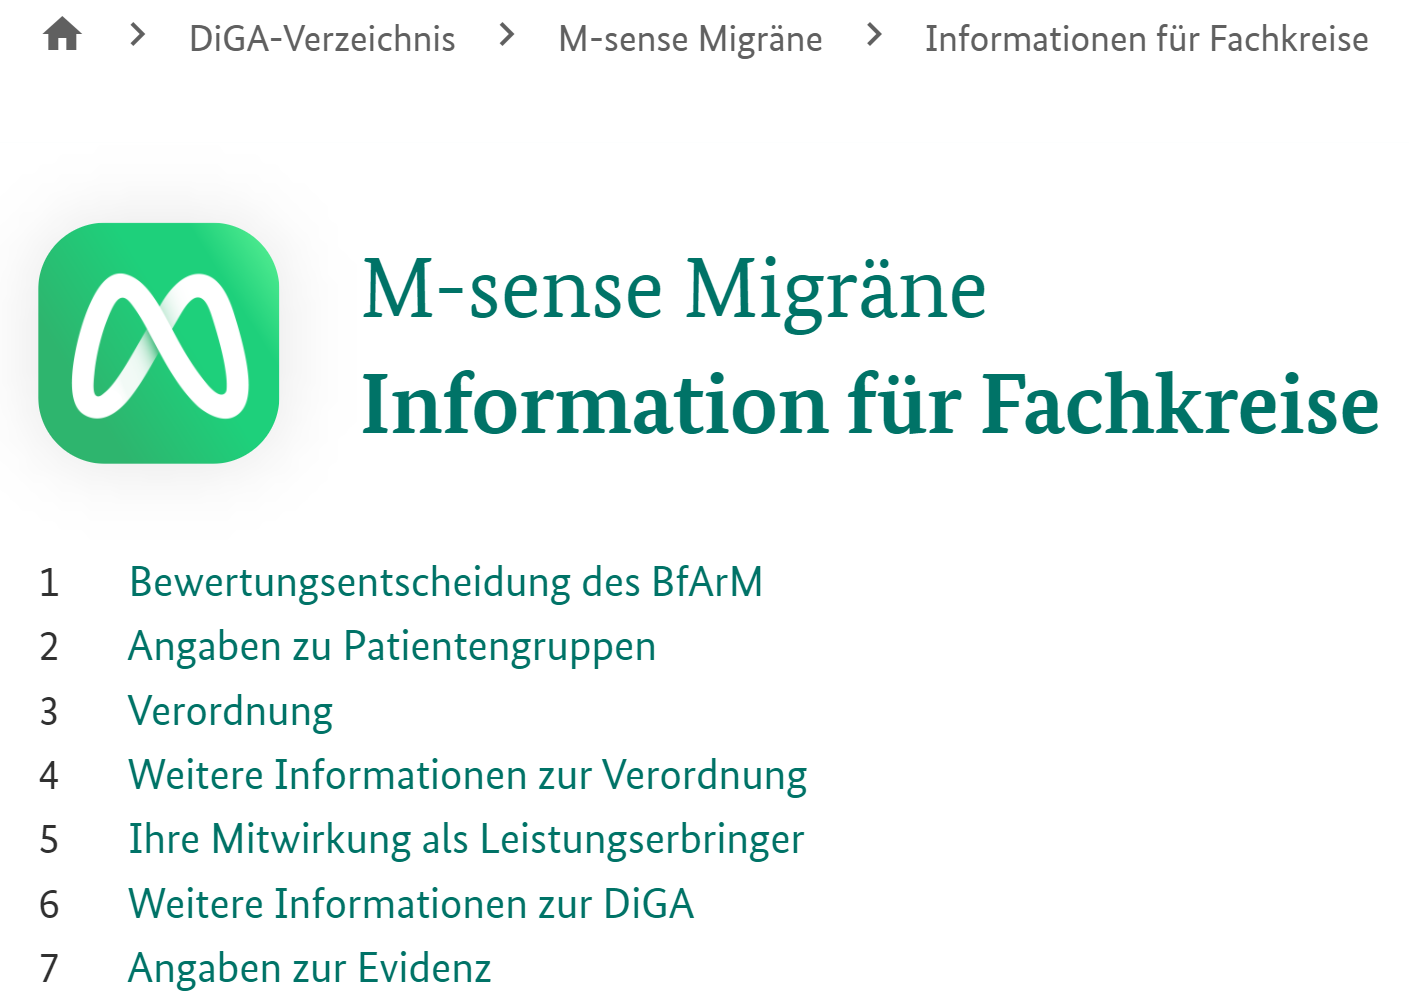
\includegraphics[width=250px, keepaspectratio]{assets/digaBSP4.png}
	\caption[DiGA-Verzeichnis - Informationsseite für Fachkreise]{DiGA-Verzeichnis - Informationsseite für Fachkreise,~Quelle:~\cite{digafachkreise}}
	\label{fig:moreInfo}
\end{figure}